\addtolength{\topmargin}{-1.59999pt}
\setlength{\headheight}{13.59999pt}

\chapter{Analysis}
\section{Introduction}
My project will be a prototype life simulator game designed for Windows devices.\\
The project will be defined as a prototype as the scope of life simulator games is extremely broad; it will not be feasible to construct a well-rounded game in the time frame set out for this project. Due to the nature of a prototype, features may be incomplete or missing altogether. In my evaluation, I will discuss what features are incomplete or missing and ways in which they could be completed.\\
The idea for this project came from playing life simulator games and wanting to improve on them by adding a competitive aspect. This will be a single score which actions in the game will determine. The aim of the game will be to get the highest score possible. I want to design and implement this game for my project because I think it will be fun as well as a challenge; I am also interested in the balancing process which I will have to go through to make my game fair for players.


\section{Computational methods my solution will contain}
This game will be amenable to being solved using a computer program because games based off of random events are complex to develop on paper and often involve a second person to act as a 'game master', the use of a computer mitigates the need for a second person.
\subsection{Abstraction}
Real life is extremely complex and has lots of different aspects to it. This game will not have every aspect of real life programmed, so I will need to use abstraction to remove the inessential aspects of life. I will also need to use abstraction to hide some of the complex algorithms from the user, including the score calculation algorithms. \newline
An area in which I will definitely be abstracting in, is in game items. The game will not have a shop or in game wardrobe, it will just be assumed that the character has clothes. A future iteration of the game may include this.
\subsection{Decomposition}
I will need to use decomposition to break down the elements of life which I have chosen to implement into small subroutines. This will maximise efficiency as I will be able to use the same well-designed subroutine many times, minimising the number of lines of code which I have to write. By using a number of subroutines, it will mean that my program can be developed further and maintained easier after I have completed this project.
\subsection{Real time processing}
Most of this game will be fundamentally based on real-time processing. Basically everything which happens will be run in real-time as the player clicks through the game. This will need to happen quickly as it is unpleasant and off putting to use software or games where there are increased wait times for seemingly simple things. \newline
The only exception to this might be the data storage, I'm not sure exactly how I will do this, it may be run parallel to the main game code.
\subsection{Calculations}
There will be a number of time calculations are used in the game. Primarily, they will be used to run the score system, calculating the scores in real time and modifying them as and when a user changes something in the game. Calculations will also be important in deciding probabilities for certain things to happen in the game; for example, there will be an algorithm which takes the character's age as an input and returns the chance of them dying. This chance will be based off of their age and a pre-determined modifier.
\subsection{Data storage}
The data generated from each round of the game will need to be able to be saved to an external (to the game) location; for example, the C drive of the computer which the game is being run on. This will enable the player to pause their game and resume at a later time or for them to share a life with their friends over a communication platform, then their friends can install the life and play through it. The game will need to have a way for the data to be re-loaded.


\section{Stakeholders}
My target audience for this game will be casual gamers, aged between 16 and 25. Generally, I have found that this is the target audience for similar games available for different platforms. This is a broad age range, covering the upper end of the teenage market and young adulthood. I have chosen this market because I think that the content of the game will be applicable and enjoyable to those who are starting out in life (teenagers) and those who have made a start in life but could stop and pick up a different track if they wanted to (young adults). \newline
The game will be suitable to the lifestyles of teenagers as it will be designed to play in short bursts, perhaps whilst they are waiting to meet up with friends or having a break from school work. It will also be engaging for teenagers with the competitive aspect allowing them to play together to get the best score at the end of a life, sharing a screenshot from the end of the game with their peers over a communication method. There won’t be any unlockable aspects, apart from character age related content in game, so if the app has to be deleted from a device, there will be no worry about losing progress after a life is completed.\newline
The game will be suitable to young adults because it will be able to be played however they want, either making use of all the features, or playing through very simply and quickly, not making use of the features which are off the main path. This will be suitable because they might want to play the game more competitively than the teenage audience, working out the optimum way to live a life to get the best score possible, beating colleagues or friends. \newline
All users will interact with the game in the same basic way. Primarily this will be through buttons on the screens, however there will be occasional keyboard input required. The use of buttons will mean this game is suitable for those using eye tracker software or those who use touch input rather than a keyboard. The game, however, will be primarily designed for interaction using a mouse and keyboard.


\section{Research}
I had initially planned to make my game for Android devices, which is no longer possible due to software restrictions. This is why my research is aimed primarily towards mobile apps. The majority of this research will translate between Android and Windows naturally, with only very minor differences explored in the design chapter. \newline
To conduct my research for my project, I will be creating a questionnaire to send to people and researching different currently available options myself.
\subsection{Questionnaire}
I will create a Google form to send out to friends and classmates who fit into my target audience and have played games like this in the past.
\subsubsection{Questions}
I have split my questions into two categories.
\begin{enumerate}
    \item Previous experiences
    \begin{enumerate}
        \item What device(s) have you used to play Life Simulator games?
        \item What life simulator games have you played?
        \item Roughly, when did you last play this game?
        \item On average, how long do you think you played these games for?
        \item What made you stop playing these games?
        \item When you have played Life simulator games, what did you like about the game? Any specific features?
        \item When you have played Life simulator games, what did you not like about the game? Any specific features?
        \item Were there any parts of the games which you found more interesting than others? If so, what were they?
    \end{enumerate}
    \item User Interface
    \begin{enumerate}
        \item Were there any parts of the user interface which you found hard to use? What were they and what was hard to use?
        \item Were there any parts of the user interface which you found easy/intuitive to use? What were they and what was hard to use?
        \item Would you prefer a light or dark theme for the app?
    \end{enumerate}
\end{enumerate}
\subsubsection{Responses to Questionnaire}
I sent the questionnaire out to the 1st year Computer Science cohort, all of whom fit into my target audience. Listed below are the results of the questionnaire.
\begin{enumerate}
    \item 
    \begin{enumerate}
        \item 
        \begin{itemize}
            \item 33.3\% - Android phone
            \item 66.7\% - iPhone
        \end{itemize}
        \item
        \begin{itemize}
            \item BitLife (4)
            \item The Sims (2)
            \item Unnamed (1)
        \end{itemize}
        \item
        \begin{itemize}
            \item 6 months ago
            \item 2 months ago
            \item May 2021
            \item Last year.
            \item 3 years ago
            \item Maybe three years ago, 2018
        \end{itemize}
        \item 
        \begin{itemize}
            \item A fortnight
            \item A couple of months
            \item 20 mins per week
            \item 4 hours
            \item Not very much
            \item 30 mins at a time
        \end{itemize}
        \item 
        \begin{itemize}
            \item Lost interest as it started to get repetitive
            \item Glitches in software and ads
            \item Boredom/Repetitive
            \item I didn\textquotesingle t find them very interesting.
            \item The time needed for waiting
            \item Boredom
        \end{itemize}
        \item 
        \begin{itemize}
            \item Entertaining dialogue with some of the random simulations
            \item I liked being able to personalise decisions to fit my life and using it to predict my future
            \item Customisation
            \item I liked customising characters in the sims.
            \item Different types of options available
            \item How it can be a different experience each time you play, the variation
        \end{itemize}
        \item
        \begin{itemize}
            \item After a while it gets repetitive, also a lot of the the more interesting/fun features were locked behind a paywall
            \item I didn’t like when they give you options and you have to pick one of them because not all of them apply so you can’t always pick something you actually want to pick
            \item Repetitive
            \item The game itself doesn\textquotesingle t really appeal to me because I didn\textquotesingle t always have to interact with it so I spent a lot of time idle while waiting for something to happen.
            \item The camera [unsure what this is referencing]
        \end{itemize}
        \item
        \begin{itemize}
            \item The minigames for things like escaping jail etc
            \item I liked being able to see that I had to work on relationships with people (maintain friendships etc).
            \item More detailed
            \item Character customisation.
            \item The building aspect
            \item Not really
        \end{itemize}
    \end{enumerate}
    \item
    \begin{enumerate}
        \item
        \begin{itemize}
            \item Not really
            \item I don’t understand what user interface means
            \item None hard to use
            \item (Bearing in mind I haven\textquotesingle t played in ages) Some of the icons weren\textquotesingle t obvious to me so I had to click around a lot to find things.
            \item Hard - free look mode
            \item Not really
        \end{itemize}
        \item 
        \begin{itemize}
            \item Most of the UI was fairly obvious as to what it did.
            \item The Buttons were simple
            \item Icons that are easily recognisable (cog for settings, house for home/menu). The buttons had a HUD so they were easy to find.
            \item Easy - guiding character
            \item Some of the larger buttons that where perfect for the size of my phone
        \end{itemize}
        \item
        \begin{itemize}
            \item 66.7\% - Dark
            \item33.3\% - Light
        \end{itemize}   
    \end{enumerate}
\end{enumerate}

\subsubsection{Reviewing Responses To The Questionnaire}
\begin{enumerate}
    \item[1d] Time played massively varied, this could be because different people have different attention spans or they could have explored different parts of the game. The time I am attracting people to my game for is not a massive concern, however it might be an interesting to engage in a focus group with those who only played for a short amount of time to understand their answer further.
    \item[1e] It seems these responses fit into three categories: bored of playing the game; bored of waiting for things to unlock (which will allow them to progress further) and software issues, whether this be an intentional pause, paywall or glitches which made users stop playing. Ads also made the game less appealing to players, however I won't be commercialising my game so this won't be a problem.
    \item[1f] The majority of these responses suggested that the variety and randomness of the games made them appealing to play, this is something I intend on recreating in my game
    \item[1g] These responses are split into two, some not liking the repetitiveness of games like this which comes naturally when you are playing lots of lives consecutively as there are only a few routes which you can go down in a virtual life; and the second responses generally dislike a paywall feature which I wouldn’t be implementing anyway.
    \item[2a] One person commented that they found the UI hard to use, I intend to use standard icons which are well used and recognised throughout the app market to counteract this, as well as use a simple icon theme to keep my app looking tidy.
    \item[2b] Most people found the UI intuitive to use, I intend to replicate this simplicity in my own way as I think that is a very key element to having a successful app.
    \item[2c] I will be making this app with a dark theme as a default.
\end{enumerate}

\subsection{Similar Games currently available}
Before I begin to design my application, I need to look at a number of other games which are available on the app market. This will help me to understand further some of the feedback which I got from my questionnaire.
\subsubsection{BitLife}
BitLife is currently available on the \href{https://play.google.com/store/apps/details?id=com.candywriter.bitlife}{Google Play Store}.\\
The description of the app on the Google Play store outlines some features which the app has, in a handwavey way.
From playing the game, I have learnt that it allows the user to age up. When the user does this it tells them about something which has happened, for example they started at a school. Then it might prompt the user as the game goes on to pick different aspects of the life, or make decisions for the character, for example, if to kiss someone or not, if to go on a date or not. I have also learnt that many of the features of the game are only accessible after the user ages up a certain amount, this is beneficial as it keeps more to the real world as a 10 year old can’t buy a house. Furthermore, there are many other features which are accessible via a menu. There is an element of morality to the game, for example when I was playing it, I was trying to make my character go on a date with many different people even though they were married, the game prevented this every time. This game also allows you to carry on playing as your child when your character dies. Throughout the life of the character, there are events which happen - for example, a family member falls ill or dies. Another feature of the game which I like is the finance management system; part of the game is having a job which earns the character money. With that money, you are then able to purchase things - for example a house or speedboat.\\
Reading the reviews of the game suggests to me that many people are happy with the game, however some suggest that there are elements which need to be improved on for the game to be more fun, for example, someone would like there to be a one month age up option so the life of the virtual character can be explored more in depth.
The app contains in-game purchases which allow ads to be removed entirely from the game.\\
The user interface of the game is relatively messy, with adverts covering parts of the game on my phone as many buttons are placed along the bottom edge of the screen. Also, lots of the menus are very small and difficult to touch accurately 
\begin{figure}[H]
    \centering
    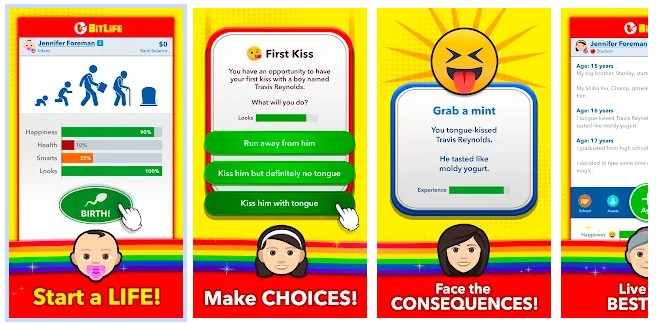
\includegraphics[width=0.9\textwidth]{images/analysis/bitLife.jpg}
    \caption{Screenshot of BitLife promotional images on the Google Play Store}
    \label{fig:bitLife}
\end{figure}

\subsubsection{Life Simulator 3}
Life Simulator 3 is currently available on the \href{https://play.google.com/store/apps/details?id=uk.playdrop.lifesimulatorpro}{Google Play store}.\\
The description of the app on the Google play store details the many elements which the game has. The main difference between this game and BitLife, is that this game allows users to create a virtual avatar whereas BitLife doesn’t.
Reading the reviews, I have learnt that there are many programmatical errors which make the game hard to play, including: when a house is sold you become “homeless” for a short while until a new house is bought, a user found that they died each time they became homeless as their health deteriorated too quickly.
Judging by the images on the Google Play store page, the user interface looks very touchscreen friendly, with big buttons and large menus where the entirety of a box is touch friendly. The images look as though the app defaults to a dark theme.
\begin{figure}[H]
    \centering
    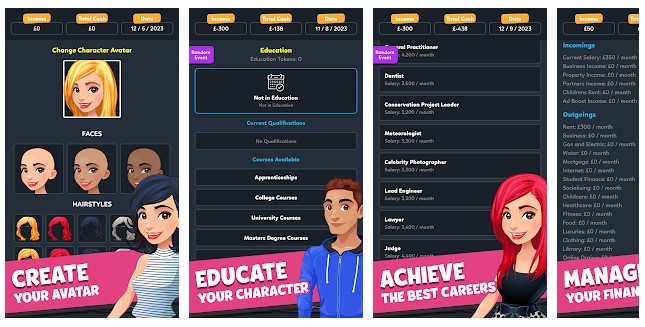
\includegraphics[width=0.9\textwidth]{images/analysis/lifeSim3.jpg}
    \caption{Screenshot of Life Simulator 3 promotional images on the Google Play Store}
    \label{fig:lifeSim3}
\end{figure}

\subsubsection{Life Simulator - Realistic Life Simulation Game}
Life Simulator - Realistic Life Simulation Game is currently available on the \href{https://play.google.com/store/apps/details?id=com.mindvacation.lifesimulator}{Google Play Store}.\\
The description of the app on the Google Play Store lists many elements which are available within the app. This app seems more modern and 'with the current times' than the others which I have looked at, containing features such as having a side hustle and a main job. It also has scenarios which set the player up to follow a specific track and achievements which can be unlocked to allow the player to do more within the app.\\
From playing this game, I have learnt that a tutorial or a clear how to play button is beneficial, which this game lacks. I spent the first 5 minutes or so trying to work out how to play the game, before stumbling across the button which makes the character older (it's a work button, not a dedicated age up button). When you do press this button, it ages you up weekly, this is shown by a tiny little dot at the top of the screen, which is not very accessible for those with a visual impairment. Also in this status bar are 3 attributes, which you have to maintain at a good level to stay alive. This is relatively challenging because to increase them, you have to spend money and when you work for money, they decrease. This is a good thing in my opinion. An improvement to this attribute display would be a percent indicator because each action has a different effect and it is hard to judge what the values in the bar are, making it hard to judge what modifier you need to apply to raise it just enough without exceeding its max value, thus wasting money. Quite a nice feature of this game, is that it doesn’t force you to follow a certain plot, even though the free version of the game forces you to pick a scenario to start the game in.\\
Reading the reviews, it seems that generally, users are happy with the game, however there are issues with the balancing of the pricing within the game.\\
The user interface of the game looks clean, with a consistent colour theme throughout the pages and greying out \& displaying a locked padlock icon for invalid buttons. It looks as though large buttons are used.
\begin{figure}[H]
    \centering
    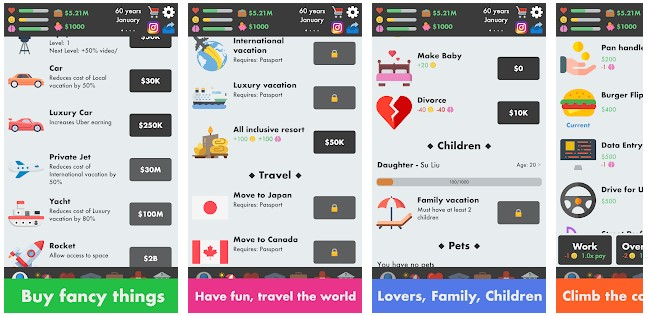
\includegraphics[width=0.9\textwidth]{images/analysis/rlsg.jpg}
    \caption{Screenshot of Life Simulator - Realistic Life Simulation Game promotional images on the Google Play Store}
    \label{fig:rlsg}
\end{figure}

\subsubsection{Reviewing Findings from Different Games}
Reviewing these similar games, it is clear that there are a few basic themes which are a constant throughout this genre of game:
\begin{itemize}
    \item Being able to make the character older
    \item Partners \& family
    \item Jobs
    \item Finance management
    \item Education
\end{itemize}
Through reviewing the games, it is clear to me there isn’t a competitive aspect to any of them. I plan on adding on to the game, through introducing a “life score”; the aim of the game is to get this score as high as possible. There will be various factors which will impact on the score.\newline
I will strive to include all of these in my final program, as well as the following which were less common amongst my research, but sound like very good ideas:
\begin{itemize}
    \item Food and diet - allowing the user to set what diet they choose for their character to dine on, this may have a financial implication if you choose for your character to eat at a hotel every day.
    \item Side Hustle - a second job which over time could progress to being the characters full time job
    \item Travelling and holidays - being able to use money earned from working to go on holiday, which improves characters attributes and opens up opportunities of finding partners with different nationalities.
\end{itemize}
There are also some elements which I really liked the look of, but will most definitely not be able to program in the time allocated for this project.

\section{Essential Features Of The Game}
\subsection{Success Criteria}
\begin{enumerate}
    \item Ageing Up
    \begin{enumerate}
        \item The game has a button which “ages up” the character
        \item As part of this process, a random event will occur (eg, family member dies, your partner wins something, you are pregnant)
        \item Some events will happen at set times (eg. finishing school)
    \end{enumerate}
    \item Relationships
    \begin{enumerate}
        \item Having a relationship with parents
        \item Having partners
        \item Marrying partners
        \item Divorcing partners
        \item Being able to pick the characters sexuality
        \item Having kids with your partner (adopted/biological)
    \end{enumerate}
    \item Crime
    \begin{enumerate}
        \item Ability to commit crime - this will be a button which will randomly generate a crime, then deduct a set amount from the lifescore.
    \end{enumerate}
    \item Employment
    \begin{enumerate}
        \item Get jobs
        \item Quit jobs
        \item The longer you stay in a job, the more \verb|jobPoints| a character will get each year. 
    \end{enumerate}
    \item Character Picker
    \begin{enumerate}
        \item At the start of each life, the user will be able to pick the character they want to play the game as. This will generate a brief backstory to the character which will crop up throughout the game (deaths of family members, key events in siblings' lives)
    \end{enumerate}
    \item Education
    \begin{enumerate}
        \item There will be a random education element to the game which will allow players to progress through school (which will have randomly generated names). Every time they complete a course or school, they get \verb|educationPoints|. 
    \end{enumerate}
    \item Saving
    \begin{enumerate}
        \item The game should be able to write the data out to a file(s) which can be loaded in during runtime to resume the game. These do not need to be readable by the user.
        \item There should be a way for the user to export the life from the game at the end of the game to a non-editable file format (eg, PDF).
    \end{enumerate}
    \item Scores
    \begin{enumerate}
        \item There should be a number of scores which the actions of the player can affect throughout the game.
    \end{enumerate}
\end{enumerate}
\subsection{Limitations of my solution}
Due to the nature of this project being a prototype which would be presented to a funding panel for assessment before further funding, there are a number of limitations of the solution.
They are outlined below.
\begin{itemize}
    \item Some aspects of the game might not be as fully fleshed out as some of the examples of similar games listed above. For example, I don’t plan on having such an intricate way of meeting partners as some of the games I played in researching; I will instead have a simple list and the player can indicate which one they wish to date;
    \item The export life function will just be to view the JSON files which the game will save data to during runtime. This will mean that definitely one element of my success criteria won't be completed;
    \item There will be a lower number of set life events, for example there will be no reference to driving lessons or other events which happen in life in a similar way;
    \item The education system will end after 6th form / college;
    \item The \verb|LifeScore| algorithm won’t be complete, however the other scores which will be the direct source of information for the \verb|LifeScore| will be complete;
    \item The marriage section of the game will not be implemented.
\end{itemize}

\section{Hardware Requirements}
As the application will be developed using Visual Studio 2019, the minimum software requirements will be the same as Visual Studios requirements:
\begin{itemize}
    \item 1.8 GHz or faster processor. Quad-core or better recommended;
    \item 2 GB of RAM; 8 GB of RAM recommended (2.5 GB minimum if running on a virtual machine);
    \item Hard disk space: Minimum of 800MB up to 210 GB of available space, depending on features installed; typical installations require 20-50 GB of free space;
    \item Hard disk speed: to improve performance, install Windows and Visual Studio on a solid state drive (SSD);
    \item Video card that supports a minimum display resolution of 720p (1280 by 720); Visual Studio will work best at a resolution of WXGA (1366 by 768) or higher.
\end{itemize}

